\documentclass{report}

% Paquetes y configuraciones adicionales
\usepackage{graphicx}
\usepackage[export]{adjustbox}
\usepackage{caption}
\usepackage{float}
\usepackage{titlesec}
\usepackage{geometry}
\usepackage[hidelinks]{hyperref}
\usepackage{titling}
\usepackage{titlesec}
\usepackage{parskip}
\usepackage{wasysym}
\usepackage{tikzsymbols}
\usepackage[spanish]{babel}

\newcommand{\subtitle}[1]{
  \posttitle{
    \par\end{center}
    \begin{center}\large#1\end{center}
    \vskip0.5em}
}

% Configura los márgenes
\geometry{
    left=2cm,   % Ajusta este valor al margen izquierdo deseado
    right=2cm,  % Ajusta este valor al margen derecho deseado
    top=3cm,
    bottom=3cm,
}

% Configuración de los títulos de las secciones
\titlespacing{\section}{0pt}{\parskip}{\parskip}
\titlespacing{\subsection}{0pt}{\parskip}{\parskip}
\titlespacing{\subsubsection}{0pt}{\parskip}{\parskip}

% Redefinir el formato de los capítulos y añadir un punto después del número
\makeatletter
\renewcommand{\@makechapterhead}[1]{%
  \vspace*{0\p@} % Ajusta este valor para el espaciado deseado antes del título del capítulo
  {\parindent \z@ \raggedright \normalfont
    \ifnum \c@secnumdepth >\m@ne
        \huge\bfseries \thechapter.\ % Añade un punto después del número
    \fi
    \interlinepenalty\@M
    #1\par\nobreak
    \vspace{10pt} % Ajusta este valor para el espacio deseado después del título del capítulo
  }}
\makeatother

% Configura para que cada \chapter no comience en una pagina nueva
\makeatletter
\renewcommand\chapter{\@startsection{chapter}{0}{\z@}%
    {-3.5ex \@plus -1ex \@minus -.2ex}%
    {2.3ex \@plus.2ex}%
    {\normalfont\Large\bfseries}}
\makeatother

\begin{document}

% Portada del informe
\title{Práctica 04. Disparadores y Vistas en SQL}
\subtitle{Administracion y Diseño de Bases de Datos}
\author{Cheuk Kelly Ng Pante}
\date{\today}

\maketitle

% Índice
\tableofcontents

% Nueva página para el primer capítulo
\cleardoublepage

% Secciones del informe
% Capitulo 1
\chapter{Realizar la restauración de la base de datos alquiler.tar}
Para realizar la restauración de la base de datos \emph{alquiler.tar}, primero debemos crear la base de datos \emph{ALQUILERDVD} y luego restaurar la base de datos con el comando \emph{pg\_restore}, como se muestra a continuación:
\begin{verbatim}
usuario@ubuntu# pg_restore -U postgres -d alquilerdvd ./alquiler.tar
\end{verbatim}

\begin{figure}[H]
  \centering
  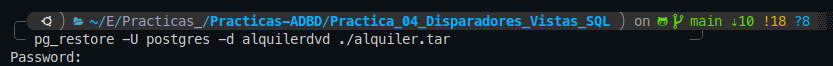
\includegraphics[scale=0.55]{img/restore_DB.png}
  \caption{Restauración de la base de datos}
  \label{fig:restauración de la base de datos}
\end{figure}

% Capitulo 2
\chapter{Identificacion de las tablas, vistas y secuencias}
Para identificar las tablas, vistas y secuencias de la base de datos \emph{ALQUILERDVD}, hay que usar la terminal interactiva de \emph{PostgreSQL} y ejecutar los siguiente comandos:
\begin{verbatim}
usuario@ubuntu# sudo -u postgres psql
postgres=# \c alquilerdvd 
alquilerdvd=# \dt
alquilerdvd=# \dv
alquilerdvd=# \ds
\end{verbatim}

\begin{figure}[H]
  \centering
  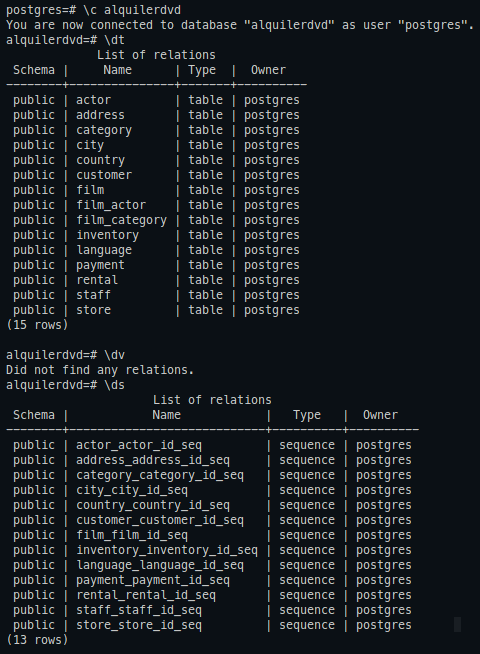
\includegraphics[scale=0.48]{img/tablas_vistas_secuencias.png}
  \caption{Identificación de las tablas, vistas y secuencias}
  \label{fig:identificación de las tablas, vistas y secuencias}
\end{figure}

% Capitulo 3
\chapter{Identifique las tablas principales y sus principales elementos}

% Tabla: actor
\CIRCLE \ \ \textbf{Tabla:} \emph{actor}
\begin{itemize}
  \item \textbf{Descripción:} Contiene la información de los actores.
  \item \textbf{Elementos:} \emph{actor\_id, first\_name, last\_name, last\_update}
\end{itemize}

% Tabla: address
\CIRCLE \ \ \textbf{Tabla:} \emph{address}
\begin{itemize}
  \item \textbf{Descripción:} Contiene la información de las direcciones.
  \item \textbf{Elementos:} \emph{address\_id, address, address2, district, city\_id, postal\_code, phone, last\_update}
\end{itemize}

% Tabla: category
\CIRCLE \ \ \textbf{Tabla:} \emph{category}
\begin{itemize}
  \item \textbf{Descripción:} Contiene la información de las categorías.
  \item \textbf{Elementos:} \emph{category\_id, name, last\_update}
\end{itemize}

% Tabla: city
\CIRCLE \ \ \textbf{Tabla:} \emph{city}
\begin{itemize}
  \item \textbf{Descripción:} Contiene la información de las ciudades.
  \item \textbf{Elementos:} \emph{city\_id, city, country\_id, last\_update}
\end{itemize}

% Tabla: country
\CIRCLE \ \ \textbf{Tabla:} \emph{country}
\begin{itemize}
  \item \textbf{Descripción:} Contiene la información de los países.
  \item \textbf{Elementos:} \emph{country\_id, country, last\_update}
\end{itemize}

% Tabla: customer
\CIRCLE \ \ \textbf{Tabla:} \emph{customer}
\begin{itemize}
  \item \textbf{Descripción:} Contiene la información de los clientes.
  \item \textbf{Elementos:} \emph{customer\_id, store\_id, first\_name, last\_name, email, address\_id, activebool, create\_date, last\_update, active}
\end{itemize}

% Tabla: film
\CIRCLE \ \ \textbf{Tabla:} \emph{film}
\begin{itemize}
  \item \textbf{Descripción:} Contiene la información de las películas.
  \item \textbf{Elementos:} \emph{film\_id, title, description, release\_year, language\_id, rental\_duration, rental\_rate, length, replacement\_cost, rating, last\_update, special\_features, fulltext}
\end{itemize}

% Tabla: film_actor
\CIRCLE \ \ \textbf{Tabla:} \emph{film\_actor}
\begin{itemize}
  \item \textbf{Descripción:} Contiene la información de los actores de las películas.
  \item \textbf{Elementos:} \emph{actor\_id, film\_id, last\_update}
\end{itemize}

% Tabla: film_category
\CIRCLE \ \ \textbf{Tabla:} \emph{film\_category}
\begin{itemize}
  \item \textbf{Descripción:} Contiene la información de las categorías de las películas.
  \item \textbf{Elementos:} \emph{film\_id, category\_id, last\_update}
\end{itemize}

% Nueva página 
\cleardoublepage

% Tabla: inventory
\CIRCLE \ \ \textbf{Tabla:} \emph{inventory}
\begin{itemize}
  \item \textbf{Descripción:} Contiene la información de los inventarios.
  \item \textbf{Elementos:} \emph{inventory\_id, film\_id, store\_id, last\_update}
\end{itemize}

% % Nueva página 
% \cleardoublepage

% Tabla: language
\CIRCLE \ \ \textbf{Tabla:} \emph{language}
\begin{itemize}
  \item \textbf{Descripción:} Contiene la información de los lenguajes.
  \item \textbf{Elementos:} \emph{language\_id, name, last\_update}
\end{itemize}

% Tabla: payment
\CIRCLE \ \ \textbf{Tabla:} \emph{payment}
\begin{itemize}
  \item \textbf{Descripción:} Contiene la información de los pagos.
  \item \textbf{Elementos:} \emph{payment\_id, customer\_id, staff\_id, rental\_id, amount, payment\_date}
\end{itemize}

% Tabla: rental
\CIRCLE \ \ \textbf{Tabla:} \emph{rental}
\begin{itemize}
  \item \textbf{Descripción:} Contiene la información de los alquileres.
  \item \textbf{Elementos:} \emph{rental\_id, rental\_date, inventory\_id, customer\_id, return\_date, staff\_id, last\_update}
\end{itemize}

% Tabla: staff
\CIRCLE \ \ \textbf{Tabla:} \emph{staff}
\begin{itemize}
  \item \textbf{Descripción:} Contiene la información de los empleados.
  \item \textbf{Elementos:} \emph{staff\_id, first\_name, last\_name, address\_id, email, store\_id, active, username, password, last\_update, picture}
\end{itemize}

% Tabla: store
\CIRCLE \ \ \textbf{Tabla:} \emph{store}
\begin{itemize}
  \item \textbf{Descripción:} Contiene la información de las tiendas.
  \item \textbf{Elementos:} \emph{store\_id, manager\_staff\_id, address\_id, last\_update}
\end{itemize}

% Nueva página 
\cleardoublepage

% Capitulo 4
\chapter{Realizacion de consultas}

% Consulta a)
\section{Ventas totales por categoria}
Para obtener las ventas totales por categoría de películas ordenadas descendentemente, se debe ejecutar la siguiente consulta:
\begin{verbatim}
alquilerdvd=# SELECT category.name, SUM(payment.amount) AS total_sales
              FROM category
              INNER JOIN film_category ON category.category_id = film_category.category_id
              INNER JOIN film ON film_category.film_id = film.film_id
              INNER JOIN inventory ON film.film_id = inventory.film_id
              INNER JOIN rental ON inventory.inventory_id = rental.inventory_id
              INNER JOIN payment ON rental.rental_id = payment.rental_id
              GROUP BY category.name
              ORDER BY total_sales DESC;
\end{verbatim}
\begin{figure}[H]
  \centering
  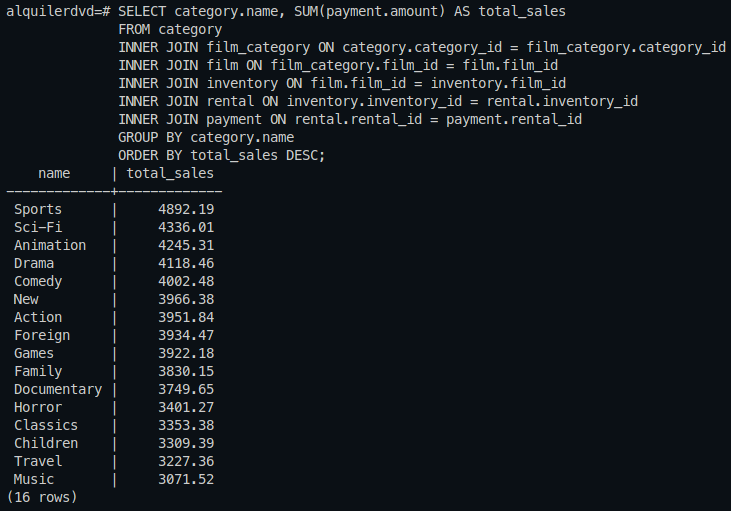
\includegraphics[scale=0.48]{img/querie_a.png}
  \caption{Ventas totales por categoria}
  \label{fig:ventas totales por categoria}
\end{figure}

% Nueva página 
\cleardoublepage

% Consulta b)
\section{Ventas totales por tienda}
Para obtener las ventas totales por tienda, donde se refleje la ciudad, el país
(concatenar la ciudad y el país empleando como separador la “,”), y el
encargado. Pusiera emplear GROUP BY, ORDER BY
\begin{verbatim}
alquilerdvd=# SELECT CONCAT(city.city, ', ', country.country) AS city_country,
              CONCAT(staff.first_name, ' ', staff.last_name) AS manager,
              SUM(payment.amount) AS total_sales
              FROM store
              INNER JOIN staff ON store.manager_staff_id = staff.staff_id
              INNER JOIN address ON store.address_id = address.address_id
              INNER JOIN city ON address.city_id = city.city_id
              INNER JOIN country ON city.country_id = country.country_id
              INNER JOIN inventory ON store.store_id = inventory.store_id
              INNER JOIN rental ON inventory.inventory_id = rental.inventory_id
              INNER JOIN payment ON rental.rental_id = payment.rental_id
              GROUP BY city_country, manager
              ORDER BY total_sales DESC;
\end{verbatim}
\begin{figure}[H]
  \centering
  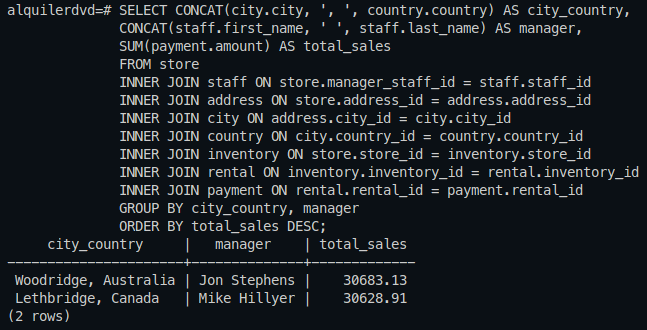
\includegraphics[scale=0.60]{img/querie_b.png}
  \caption{Ventas totales por tienda}
  \label{fig:ventas totales por tienda}
\end{figure}

% Nueva página 
\cleardoublepage

% Consulta c)
\section{Lista de películas}
Para obtener una lista de películas, donde se reflejen el identificador, el
título, descripción, categoría, el precio, la duración de la película,
clasificación, nombre y apellidos de los actores (puede realizar una
concatenación de ambos). Pusiera emplear GROUP BY
\begin{verbatim}
alquilerdvd=# SELECT film.film_id, title, description, category.name AS category_name, 
              rental_rate, length, rating,
              actor.first_name || '  ' || actor.last_name AS actor_name
              FROM film
              INNER JOIN film_actor ON film.film_id = film_actor.film_id
              INNER JOIN actor ON film_actor.actor_id = actor.actor_id
              INNER JOIN film_category ON film.film_id = film_category.film_id
              INNER JOIN category ON film_category.category_id = category.category_id
              ORDER BY film_id;
\end{verbatim}
\begin{figure}[H]
  \centering
  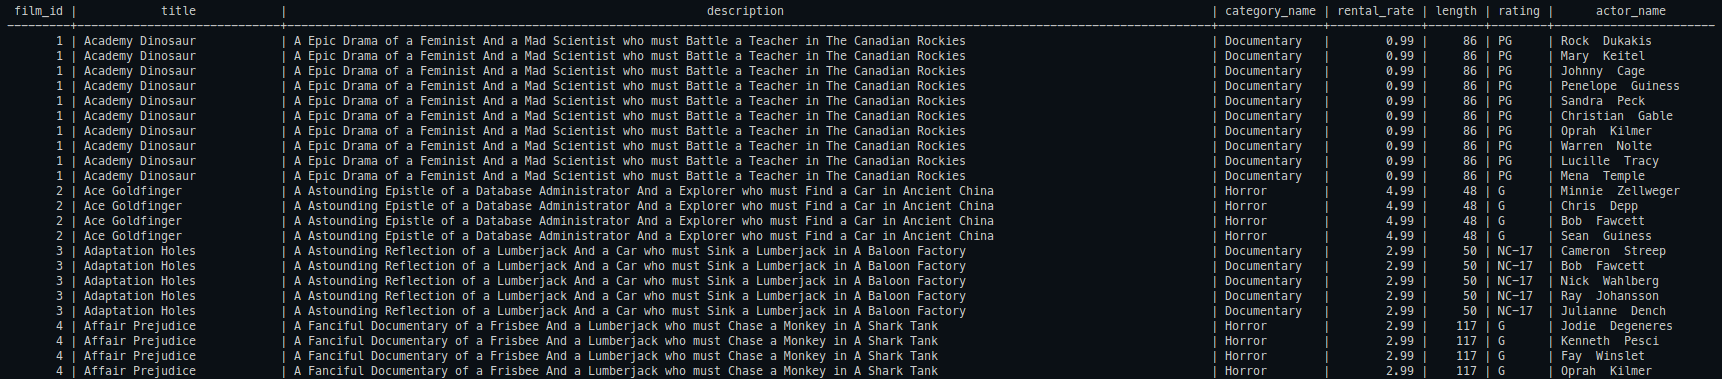
\includegraphics[scale=0.28]{img/querie_c.png}
  \caption{Lista de películas}
  \label{fig:lista de películas}
\end{figure}

% Nueva página 
\cleardoublepage

% Consulta d)
\section{Información de los actores}
Para obtener la información de los actores, donde se incluya sus nombres y
apellidos, las categorías y sus películas. Los actores deben de estar
agrupados y, las categorías y las películas deben estar concatenados por
“:”
\begin{verbatim}
alquilerdvd=# SELECT actor.first_name || ' ' || actor.last_name AS actor_name,
              string_agg(DISTINCT category.name, ':') AS categories,
              string_agg(DISTINCT film.title, ':') AS films
              FROM actor
              INNER JOIN film_actor ON actor.actor_id = film_actor.actor_id
              INNER JOIN film_category ON film_actor.film_id = film_category.film_id
              INNER JOIN category ON film_category.category_id = category.category_id
              INNER JOIN film ON film_category.film_id = film.film_id
              GROUP BY actor_name;
\end{verbatim}
\begin{figure}[H]
  \centering
  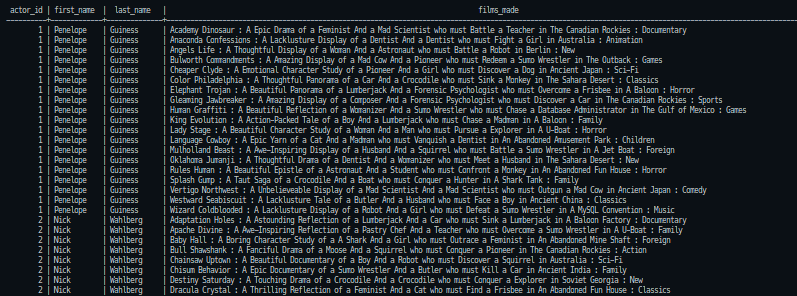
\includegraphics[scale=0.60]{img/querie_d.png}
  \caption{Información de los actores}
  \label{fig:información de los actores}
\end{figure}

% Nueva página
\cleardoublepage

% Capitulo 5
\chapter{Vistas de las consultas realizadas}
Para crear las vistas de las consultas realizadas se usará el prefijo \emph{VIEW} para identificarlas. A continuación se muestra el código de cada vista:

% Vista a)
\section{Ventas totales por categoria}
Para crear la vista de las ventas totales por categoría, se debe ejecutar la siguiente consulta:
\begin{verbatim}
alquilerdvd=# CREATE VIEW total_rent_per_category A
              SELECT category.name, SUM(payment.amount) AS total_sales
              FROM category
              INNER JOIN film_category ON category.category_id = film_category.category_id
              INNER JOIN film ON film_category.film_id = film.film_id
              INNER JOIN inventory ON film.film_id = inventory.film_id
              INNER JOIN rental ON inventory.inventory_id = rental.inventory_id
              INNER JOIN payment ON rental.rental_id = payment.rental_id
              GROUP BY category.name
              ORDER BY total_sales DESC;
\end{verbatim}

% Vista b)
\section{Ventas totales por tienda}
Para crear la vista de las ventas totales por tienda, se debe ejecutar la siguiente consulta:
\begin{verbatim}
alquilerdvd=# CREATE VIEW total_rent_per_store AS
              SELECT CONCAT(city.city, ', ', country.country) AS city_country,
              CONCAT(staff.first_name, ' ', staff.last_name) AS manager,
              SUM(payment.amount) AS total_sales
              FROM store
              INNER JOIN staff ON store.manager_staff_id = staff.staff_id
              INNER JOIN address ON store.address_id = address.address_id
              INNER JOIN city ON address.city_id = city.city_id
              INNER JOIN country ON city.country_id = country.country_id
              INNER JOIN inventory ON store.store_id = inventory.store_id
              INNER JOIN rental ON inventory.inventory_id = rental.inventory_id
              INNER JOIN payment ON rental.rental_id = payment.rental_id
              GROUP BY city_country, manager
              ORDER BY total_sales DESC;
\end{verbatim}

% Nueva página
\cleardoublepage

% Vista c)
\section{Lista de películas}
Para crear la vista de la lista de películas, se debe ejecutar la siguiente consulta:
\begin{verbatim}
alquilerdvd=# CREATE VIEW films_list AS
              SELECT film.film_id, title, description, category.name AS category_name, 
              rental_rate, length, rating,
              actor.first_name || '  ' || actor.last_name AS actor_name
              FROM film
              INNER JOIN film_actor ON film.film_id = film_actor.film_id
              INNER JOIN actor ON film_actor.actor_id = actor.actor_id
              INNER JOIN film_category ON film.film_id = film_category.film_id
              INNER JOIN category ON film_category.category_id = category.category_id
              ORDER BY film_id;
\end{verbatim}

% Vista d)
\section{Información de los actores}
Para crear la vista de la información de los actores, se debe ejecutar la siguiente consulta:
\begin{verbatim}
alquilerdvd=# CREATE VIEW actor_list AS
              SELECT actor.first_name || ' ' || actor.last_name AS actor_name,
              string_agg(DISTINCT category.name, ':') AS categories,
              string_agg(DISTINCT film.title, ':') AS films
              FROM actor
              INNER JOIN film_actor ON actor.actor_id = film_actor.actor_id
              INNER JOIN film_category ON film_actor.film_id = film_category.film_id
              INNER JOIN category ON film_category.category_id = category.category_id
              INNER JOIN film ON film_category.film_id = film.film_id
              GROUP BY actor_name;
\end{verbatim}

% Nueva página
\cleardoublepage

% Capitulo 6
\chapter{Análisis del modelo y restricciones \emph{CHECK}}
Dentro del modelo de la base de datos \emph{ALQUILERDVD} se puede observar que existen tablas que emplean atributos
que hacen uso de identificadores de tuplas que se encuentran en otras tablas, por lo que se puede decir que existen
relaciones entre las tablas. 

Se podrían implementar restricciones \emph{CHECK} que se encarguen de comprobar que dichos
números de identificación existan en las tablas relacionadas, de esta manera se asegura que no se inserten datos que
no existan en la base de datos. Por ejemplo, en la tabla \emph{film\_actor} se puede implementar una restricción
\emph{CHECK} que compruebe que el identificador de la película exista en la tabla \emph{film} y que el identificador
del actor exista en la tabla \emph{actor}:
\begin{verbatim} 
ALTER TABLE film_actor
ADD CONSTRAINT CHECK (film_id IN (SELECT film_id FROM film) AND
                      actor_id IN (SELECT actor_id FROM actor));
\end{verbatim}

Otra restricción que se podría implementar es que el identificador de la película en la tabla \emph{film\_category}
exista en la tabla \emph{film}:
\begin{verbatim}
ALTER TABLE film_category
ADD CONSTRAINT CHECK (film_id IN (SELECT film_id FROM film));
\end{verbatim}

% % Nueva página
% \cleardoublepage

% Capitulo 7
\chapter{Funcionamiento del trigger}
El siguiente trigger:
\begin{verbatim}
last_updated BEFORE UPDATE ON customer FOR EACH ROW EXECUTE
PROCEDURE last_updated()
\end{verbatim}

Se encarga de actualizar el atributo \emph{last\_update} de la tabla \emph{customer} cada vez que se actualice una
tupla de la tabla \emph{customer}. Para probar el funcionamiento del trigger, se ejecutará la siguiente consulta:
\begin{verbatim}
alquilerdvd=# UPDATE customer SET first_name = 'Cheuk' WHERE customer_id = 1;
\end{verbatim}

Para comprobar que se ha actualizado el atributo \emph{last\_update} de la tupla con \emph{customer\_id} igual a 1,
se ejecutará la siguiente consulta:
\begin{verbatim}
alquilerdvd=# SELECT last_update FROM customer WHERE customer_id = 1;
\end{verbatim}

\begin{figure}[H]
  \centering
  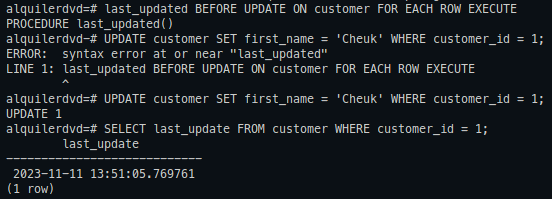
\includegraphics[scale=0.60]{img/trigger.png}
  \caption{Funcionamiento del trigger}
  \label{fig:funcionamiento del trigger}
\end{figure}

% Nueva página
\cleardoublepage

% Capitulo 8
\chapter{Construcción de un disparador}
Para construir un disparador que se encargue de guardar en una nueva tabla creada por el usuario en la fecha de cuando 
se insertó un nuevo registro en la tabla \emph{film}, se debe ejecutar la siguiente consulta:
\begin{verbatim}
alquilerdvd=# CREATE TABLE updated_table_film (
              id_updated_table_film SERIAL PRIMARY KEY,
              last_update TIMESTAMP NOT NULL
              );
\end{verbatim}


\end{document}